\chapter{Algorithm Recognition}
\label{chap:ch3}

\section{Supervised Learning}
Supervised Learning is the field of machine learning in which the model is trained against known label or tags. The model for a given data point can't predict any thing not mentioned in the vocabulary. There are some fixit numbers of label for a machine learning task.

\subsection{Background}
In case of the image classification, there is a image dataset and each image is labeled. We run the training using the given images as the input and predict the image label. Given the true value and predicted value, we calculate the loss with is used to generate gradient.

\subsection{Methodology}
On the similarly ground, We are trying to do algorithm recognition. Here given the bunch of the program, we want to predict to give algorithm class the program belong to.

We developed an classifier in TensorFlow which can classify the program respectively. 
\subsubsection{DataSet}
We have selected the POJ-104 dataset\ref{} for our experiments. It has 104 type of different program which acts like class or label and each class has approximately ~500 programs. We have splitted this dataset into 3:1:1(training:testing:validation).

\subsection{Embedding Generation}
I have used IR2Vec to generate the embedding for the programs. For each program, we get a 300 dimension vector and it's corresponding label.

\subsection{Model Architecture}
The first input layer expects a 300-dimension vector which is followed by simple three layered Multi-Level Precptron(MLP) with a softmax layer for output. The Categorical cross entropy Loss is used as the loss function and Adam as the optimizer. The whole training run for 100 epochs.

\subsection{Results}
% Table~\ref{tab-acc} rather than table~\ref{tab-acc}.
\begin{table}[h]
\begin{tabular}{l l l l}
\hline
Percentage & TBCNN & inst2vec &  Ours\\
\hline
Accuracy(\%) & 94 & 94.83 & 96.2 \\
\hline
\end{tabular}
\centering
\caption{Compare the accuracy percentage.}
\label{tab-acc}
\end{table}

\subsection{Visual Technique}
As mentioned above have 300 dimension vector and it reduce it's dimension to 2 dimensions using t-SNE\cite{}. Points which are similar to each other meant to be near to each other. The effectiveness of the encoding different instance to time during training is shown.

\begin{figure}[h]
    % \centering
\begin{subfigure}[b]{0.3\textwidth}
%   \centering
  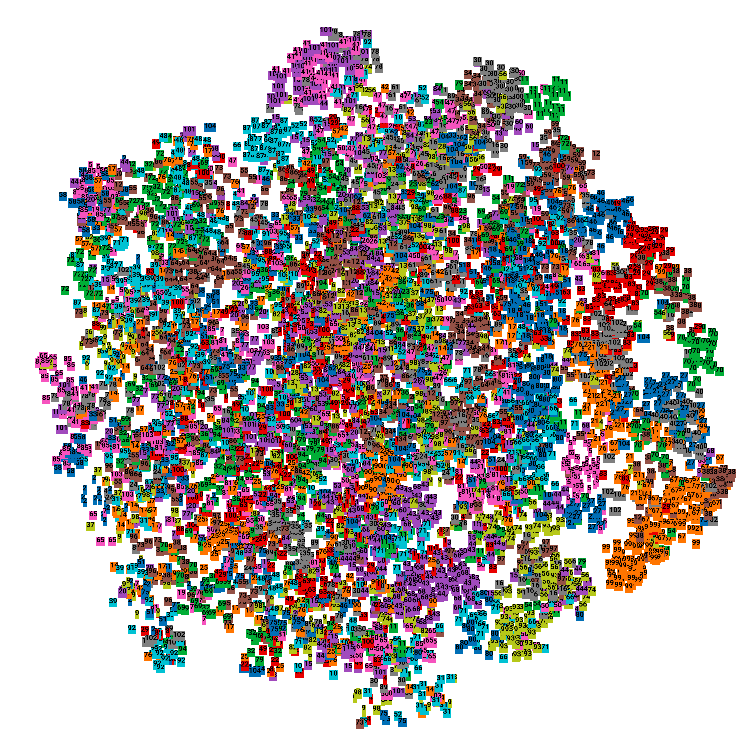
\includegraphics[width=\textwidth]{figures/untrained.png}  
  \caption{Untrained}
  \label{fig:0e}
\end{subfigure}
\hfill
\begin{subfigure}[b]{0.3\textwidth}
%   \centering
  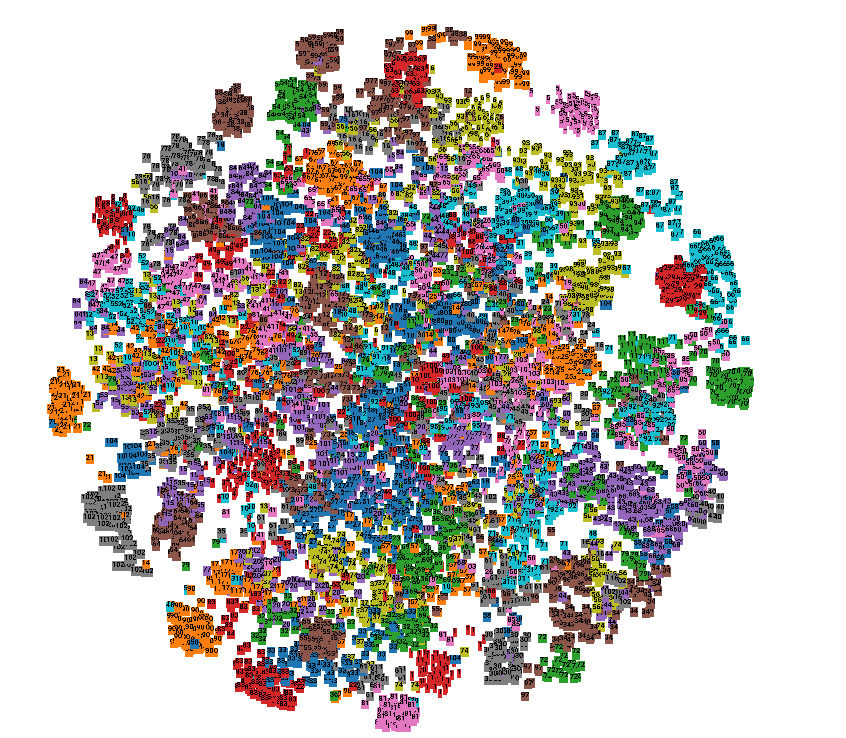
\includegraphics[width=\textwidth]{figures/5e_tsne.png}  
  \caption{After 5 Epochs}
  \label{fig:5e}
\end{subfigure}
\hfill
\begin{subfigure}[b]{0.3\textwidth}
%   \centering
  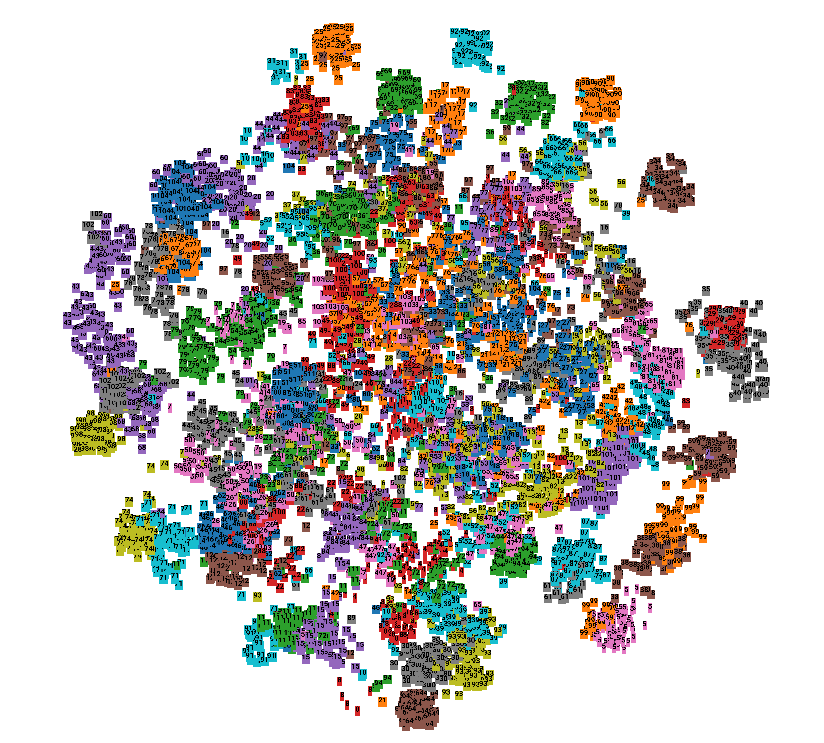
\includegraphics[width=\textwidth]{figures/full_tsne.png}  
  \caption{After 100 Epochs}
  \label{fig:100e}
\end{subfigure}
    \caption{Comparison of cluster at different instant}
    \vspace*{-\baselineskip}
    \label{fig:clusters}
\end{figure}

\begin{itemize}
    \item In Fig.~\ref{fig:0e}, we show the untrained data. It can be seen that points of similar labels are grouped together to some extent, though the clusters are not formed distinctly.
    % \vspace*{-0.4cm}

% It is a well accepted fact that the weights of the penultimate layer of the neural network represe the representation of 
% After training the classification model with the training data points for 5 epochs, we obtain the 

    \item In Fig.~\ref{fig:5e}, we show the plot formed by the learned output vectors that were taken from the last layer of the classification model after 5 epochs of the training for the same test data points. As it can be seen, on a minimalistic training, they quickly form better clusters.
    %   \vspace*{-0.4cm}
    \item At the end of training, after 100 epochs, the points form more distinct clusters as shown in Fig.~\ref{fig:100e}.
\end{itemize}

% Unsupervised Learning started
\section{Unsupervised Learning}


\subsection{Background}
Unsupervised learning is the machine learning technique that is used to train the model without labels. The clustering algorithm like KNN, K-means, hierarchical clustering, and others. 
	Learning used to happen based upon minimizing the intra-cluster distance and maximizing the inter-cluster distances. Similar data points stay near a similar point and far from the non-similar ones. This can be used for the inference of the unseen classes.
	
	As the Fig[2], given the set of unlabelled program and pass them through a  machine learning model. The model will try to form clusters of similar programs during the training. After training is done, we perform inference on the model, it try to assign the program to the best-suited cluster. This is a schematic diagram of the flow for better understanding.

	Few short learning is a way of unsupervised learning in which while inference there is some data point in which the trained model adjusts the final prediction.

\begin{figure}[t]
    \centering
    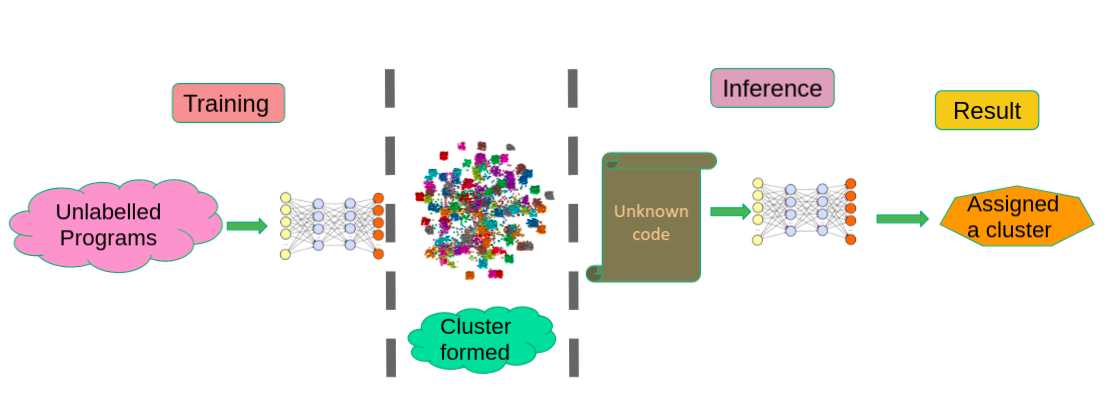
\includegraphics[scale=0.4]{figures/chapter-2/unsupervised.png}
    \caption{Algorithm Recognition in Unsupervised Way}
     \label{fig:unsupervised-background}
\end{figure}

\subsection{Few short learning}
	    It is a type of unsupervised learning, in which the training phase has two sets i.e support set and a Query set. The training happens in task. Each task consist of N classes and K datapoint in the support set and N classes in the support set. Each task has a mutually exclusive set i.e. all the N classes are not part of another task.
% 	Training

    A task is given to the model and support set is passed to the model. Now to see how much the model learns after first task, we run it on the query set for which we knew the label. The datapoint belonging to same class should lie near to each other. In the example fig[], Cat in the query set of task 1 should lie near the cat cluster of the support set and respectively for other classes.
	
	The Loss function is formulated in terms of the distance metic. If the query set is far apart during training then more is the loss and that needs to backpropagate for the better learning of the next task or batch.

\begin{figure}[t]
    \centering
    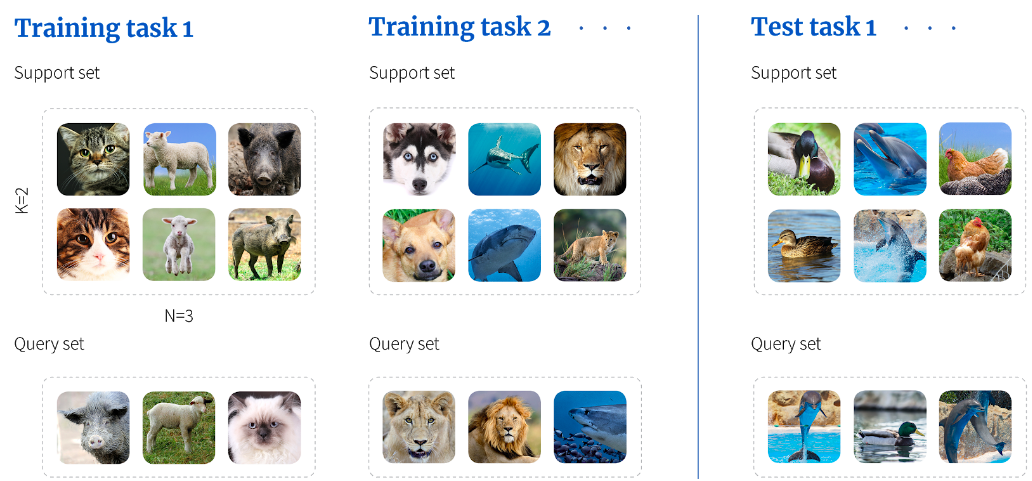
\includegraphics[scale=0.4]{figures/chapter-2/unsupervised_few_short.png}
    \caption{Few Short Learning Example}
     \label{fig:unsupervised-fewShort}
\end{figure}

\subsection{Program categorization for unseen programs}
Inspring from the work mentioned above, we want to apply the same technique to the programs. We make the required changes to the ProtoNet codebase to adapt to our work. 

\begin{figure}[t]
    \centering
    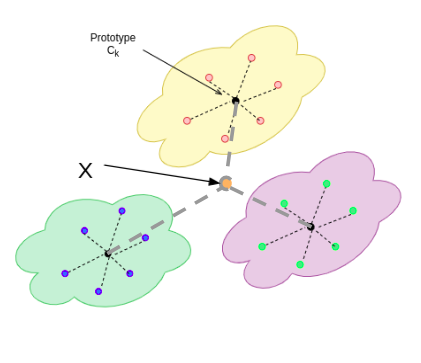
\includegraphics[scale=0.5]{figures/chapter-2/prototypes.png}
    \caption{Prototypes}
     \label{fig:unsupervised-prototypes}
\end{figure}

\subsection{ProtoNet}
\subsubsection{Prototype}
During the training phase when the support set is passed the model. Each class forms an aggregate point from other participating points and known as the prototype.
 
\subsubsection{Loss function}
During the training phase, datapoint from form each class of the Query set to evaluated against the respective prototype. The loss function forms the probability distribution of the point to which class it lies. Less is the distance, near is the point.
    		           

\subsection{Dataset}
We have selected the POJ-104 dataset\ref{} for our experiments. It has 104 type of different program which acts like class or label and each class has approximately ~500 programs. We have split this dataset into Train: Test: Val →  1-80 classes (80): 81-94 classes (14): 95-104 classes (10).

\subsection{Model Architecture}
The implementation was done using PyTorch in python. The first input layer expects a 300-dimension vector which is followed by a simple three-layered Multi-Level Perceptron(MLP) with a softmax layer for output. The Prototypical is used as the loss function and Adam optimizer. The whole training runs for 100 epochs.

\subsection{Results}

\begin{table}[h]
\begin{tabular}{lllll}
\hline
\multirow{2}{*}{\textbf{POJ Experiment}} & \multicolumn{2}{l}{\textbf{5 ways}} & \multicolumn{2}{l}{\textbf{10 ways}} \\
 & \textbf{1 Shot} & \textbf{5 Shot} & \textbf{1 Shot} & \textbf{5 Shot} \\
\hline
Test Accuracy \% & 78.47 & 89.66 & 80.9 & 91.27 \\
\hline
\end{tabular}
\centering
\caption{Compare the accuracy percentage.}
\label{unsupervised-acc}
\end{table}